\documentclass{article}
\usepackage{graphicx}

\begin{document}

\title {Robot programming for dummies}
\author {Tessa Lau \\
Willow Garage \\
Menlo Park, CA USA \\
{\tt tlau@willowgarage.com}
}
\maketitle

I never thought I would be a roboticist. In grad school, our robotics team spent months teaching little robot dogs to play soccer and solving other seemingly simple problems. Far better to work in the world of software, I figured, where the systems I built could make a real difference in people's lives. Software robots would automate repetitive tasks in computer use and free people from mundane work. End user programming would enable millions of ordinary computer users to customize and adapt systems to their own needs.

But that world is changing. Computing has moved off the desktop and into the smartphones, smart environments, and the world aronud us. Innovation is happening in the real world, using computing to effect physical change in our environment. The past decades have seen industrial robots increase manufacturing efficiency on the factory floor. Even more, we are now seeing robots tackle tasks from our daily lives. Robotic vacuum cleaners are changing the way we clean our homes. Robotic lawnmowers keep the yard tidy without having to lift a finger. Nest's robotic thermostat learns your habits and keeps your home at the optimal temperature. Google's driverless car could change the way we commute.

All these innovations have become possible through multiple advances: in sensor technology, which robots use to perceive the world around them; in planning and navigation, which enable robots to move around in the world unaided; in human-safe motion controllers, which let robots move their limbs without endangering the people around them; in the ROS open source robot operating system, which enables roboticists to build on each others' work without starting from scratch; and many more advances in the broader field of robotics.

Yet the holy grail of personal robotics remains elusive. When will we have our own Rosie the Robot (from the Jetsons cartoon) to take over housekeeping chores? When will disabled adults have robot helpers to assist them in activities of daily living? All of these advances in robotics still fall short of the goal of creating personal robots that can do whatever we want them to do.

Actually, the problem is not that robots {\em can't} do what we want them to do. The problem is that it's too difficult to {\em tell} robots what we want them to do. The first company to crack the nut of end user robot programming will corner the market on household robots. Human-robot interaction is the missing link for widespread personal robotics.

\section{Case study: Robots for Humanity}

One potential use case for personal robotics will be in-home care and assistance for disabled adults. The Robots for Humanity project, a collaboration between Willow Garage and Georgia Tech, aims to develop technology that enables persons with motor impairments to perform personal care tasks that they otherwise might not have been able to perform without assistance, such as picking up a dropped object, fetching a towel, or even scratching an itch. Its first prototypes have enabled Henry Evans, a mute quadriplegic, to act in the world for the first time since a brainstem stroke left him paralyzed. Limited to the ability to move a single finger, Henry has been able to instruct Willow Garage's PR2 robots to open cabinets, fetch food from the refrigerator, and even dole out candy to trick-or-treating kids on his behalf.

Yet our experience with Robots for Humanity underscores how difficult it is for ordinary mortals to instruct robots what to do. Even using state-of-the-art robot visualization software developed at Willow Garage, simple tasks such as opening a cabinet door could take Henry upwards of 15 minutes to accomplish.  While Henry has only limited interaction capabilities due to motor impairment, he also has incredible motivation. Ordinary consumers, on the other hand, while fully able-bodied, may not share the same perseverance in programming robots.

Until users are able to instruct robots quickly and with low effort, personal robotics will be limited to niche markets.  Why is end user robot programming so challenging? Several compounding factors make it more difficult than normal computer use.

\section{The state of the art}

% History of ROS
% Invented by Willow Garage, new operating system for diverse robots
% Current reach
% Running on robots from PR2 to android-powered XXX
% Provides very rich control substrate for programming the behavior of complex robots

The Robot Operating System is one of the software advances that supports the rapid development of new robotics technology.  First developed in 2007 at the Stanford Articifial Intelligence Laboratory, ROS was maintained by Willow Garage from 2008-2013 and has recently transitioned into the stewardship of the non-profit Open Source Robotics Foundation.

ROS provides a distributed publish/subscribe messaging platform for a collection of {\em nodes} to communicate with each other. Each node encapsulates a small amount of robot functionality, and interfaces with the rest of the ROS ecosystem to make that functionality available through a common interface. For example, ROS nodes exist to stream video from webcams, control the motors in robot arms, plan a path from one point to another, and recognize graspable objects in an image.

Before ROS, roboticists had to create the software to control their robots from scratch, each doing the same work to create device drivers and rebuild libraries for their specific robot's hardware.  Now, ROS has been ported to around 100 different models of robots worldwide\footnote{http://www.ros.org/wiki/Robots}, enabling roboticists to quickly bring a new robot model online.

\begin{figure}[tbh]
\scalebox{0.15}{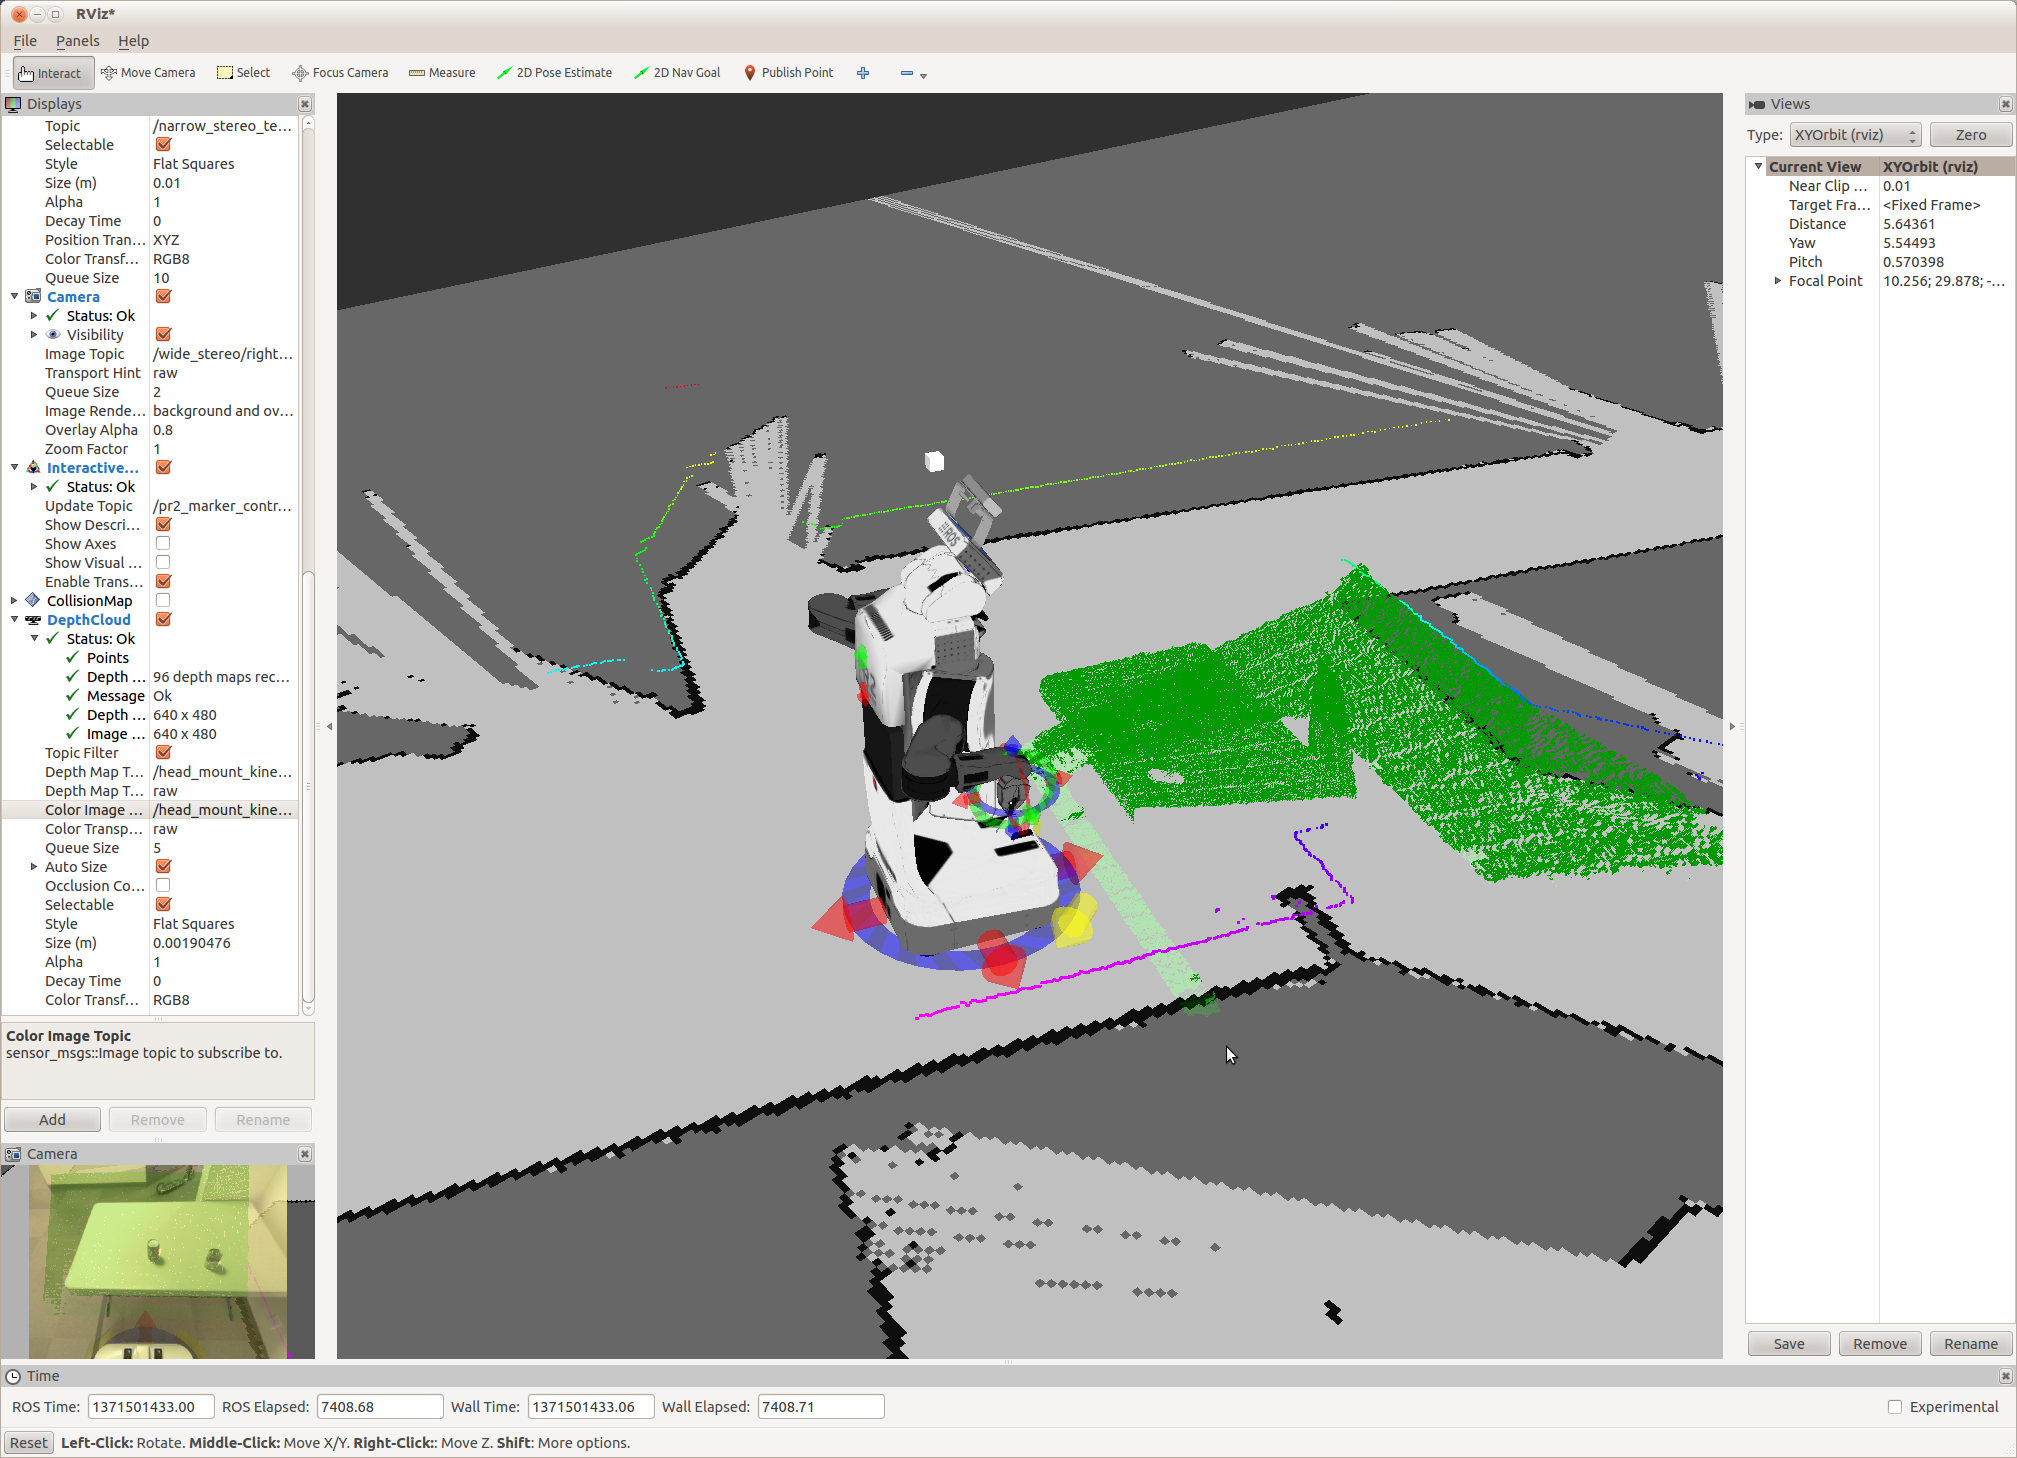
\includegraphics{rviz.png}}
\caption{RViz interface for controlling robots}
\label{rviz}
\end{figure}

However, ROS provides a fairly low-level interface to robot control. Designed for roboticists, the RViz interface (Figure~\ref{rviz}) displays all the sensor feeds coming from the robot and lets one send low-level motion commands to the robot such as rolling forward or rotating the shoulder joint. In the figure, a robot is shown examining objects on a table in front of it. The green pattern represents the data from a depth sensor mounted on the robot's head, whereas the purple line represents the walls detected by a laser rangefinder mounted on the robot's base. The tricolored axes display the various coordinate frames in use, and the gray floor displays the map the robot uses for navigation. (TODO: display costmaps, TF axes)

This interface, while well suited for roboticists who need to examine the low-level sensor data and messages being processed by the robot, is not very user-friendly. It also illustrates some of the difficulties inherent in robot programming, which I will detail next.

\section{High dimensionality}

% Robot arms have 7DOF
% grasps require 6D
% world is 3D
% quaternions, matrix manipulation
% specialized I/O devices

Unlike traditional computer interfaces which are restricted to two dimensions, robot control requires manipulating objects in a three-dimensional world. Visualizing a 3D world on existing 2D displays requires the extra dimension to be projected down into two dimensions, giving rise to the popular ``first person shooter'' style of interface. These interfaces display the world as perceived from a virtual camera, where objects can be occluded by other objects. Additional camera controls are needed to pan/zoom around the space to overcome occlusion, and these controls can be nonintuitive to non-expert computer users.

High dimensionality is even more important in specifying how to grasp and place objects in the world. A solid object has six degrees of freedom: three degrees to specify its position, and another three to specify its rotation. The human arm, and the most advanced robotic arms, have seven degrees of freedom.  Many robot arm control interfaces ask users to independently specify joint angles for each of those seven degrees of freedom. These interfaces are cumbersome because the joints are interdependent: setting the angle of one joint, such as the elbow, dictates what angles are possible for the shoulder and vice versa.

Expert roboticists manage high-dimensionality by representing the world in terms of {\em reference frames} (coordinate systems that are defined relative to particular robot part, such as the base or the head-mounted camera) and {\em quaternions} (a matrix that represents position and orientation in 3D space relative to a reference frame). Robot joint positions are typically specified relative to their own reference frame; for example, a robot's wrist, which is located at the end of its arm, can be commanded to rotate around the axis that is aligned with the robot's forearm (similar to the motion we use to screw in a light bulb). Calculating the absolute position of a robot's hand (for example, to determine whether it is near the door handle) requires a series of complex matrix calculations starting from the position of its base, through its shoulder, and all the joints, down to the hand. The opposite problem, calculating the joint positions required to get the hand to a particular position, is called {\em inverse kinematics} and is typically solved using heuristic approximation methods. More generally, techniques for {\em motion planning} calculate whole trajectories of how to move an arm from a starting location to an ending location, using inverse kinematics to compute trajectories for each of the joints in turn.

Toolkits for doing automatic motion planning are on the verge of becoming mature, simplifying the problem of robot arm control from how the arm should move in fine-grained detail to specifying only the high-level target position and orientation. Yet the challenge of specifying that 6-DOF target position and orientation still remains, and this will continue to be a challenge for easy-to-use robot interfaces that work with existing 2D displays and input devices.

\section{Concurrency}

% ROS nodes
% multiple parts of robots (head, arms, base)
% callbacks, coroutines, threads

Robots are complex beings full of many moving parts. For example, Willow Garage's robotic research platform, the PR-2, has two independently controlled arms, a head that can pan and tilt, a torso that can be raised and lowered, and a base that can move and turn in all directions. Each of these parts must be controlled independently in order to orchestrate a desired robotic behavior.

Concurrent programming is notoriously difficult even for professional programmers due to the possibility for race conditions and the complexity of reasoning about what the program does. Most robot programs can be simplified by only controlling one moving part at a time: first move the base, then raise the torso, then position the left arm, then position the right arm, finally open the cabinet. For many tasks this is a reasonable solution. However there is a subset of human tasks for which we need multiple parts moving simulateously, such as picking up a heavy or bulky object with two hands, or turning one's head to look where one is going.

End user programming systems have tried to simplify the problem of concurrency. One approach used is visualizing the different components on a timeline. This approach is popular with media creation tools such as Apple's GarageBand or Autodesk's 3D Studio Max. A different approach, taken by visual programming languages such as Scratch, enable programmers to define multiple blocks of code within the workspace, all of which run simultaneously and independently.

A second option for concurrency is to reduce the end user's need to write concurrent programs by defining new primitives that cover the common cases where concurrency is needed.  For example, a robot navigation algorithm may include the ability to turn the robot's head to look in the direction of motion, eliminating the need for the user to specify this complex behavior.  As another example, a two-armed robot could have both arms linked in a mirror configuration so that a command to move one arm would cause the other to mirror its motion, thus enabling the robot to pick up symmetric objects with two hands.

Even with higher-level primitives, there will still be a need for concurrent robot programming at a higher level. One form this will take is for background tasks, such as specifying that a robot should try to tidy up the room in between (or during) its other assigned chores. Supporting high level concurrency will introduce new problems, such as task prioritization (should it interrupt its task of bringing you a beer to clean up a wine spill on carpet?).

\section{Uncertainty}

% World changes out from under you
% Hardware fails
% Incomplete world models
% Bayesian methods, probabilities

Another challenge that robot programmers face is specifying how the robot should behave in an uncertain world. The world is constantly changing: any model that a robot could build of where things are located will be obsolete by the time it turns around. People walk around, objects get lost, furniture gets moved. Moreover, limitations in current sensing technology make it difficult to build a perfectly accurate model of the world. For example, differences in lighting make the same object look very different to an RGB camera. Therefore a robot cannot necessarily trust what it perceives, and it must be able to deal with the possibility that what it thinks is true is not actually true.

In addition, robot hardware itself often produces unpredictable results. Unlike software, mechanical parts can slip, burn out, or break. Giving a robot the same instruction multiple times may or may not result in the same result each time.

What does this mean for robot programmers? Robot programs must have mechanisms in place to deal with uncertain truth. Rather than simplying instructing the robot to pick up an object, the program must specify what to do if the object is not {\em where} it thinks it is, is not {\em what} it thinks it is, or if the robot fails to perform the desired grasp.

In order to deal with these various types of uncertainty, professional programmers can learn to use probabilistic models such as Bayesian networks or HMMs, or they write code with lots of built-in error checking. However, casual programmers who just want a robot to perform a job in the home would find it burdensome to have to think through all the ways in which the robot could fail, and specify what the recovery strategy should be in each case.

Most end user programming systems to date ignore the problem of uncertainty. Some can get away with this because they operate in a simulated world (such as Scratch). Others, which deal with uncertainty in the form of network requests timing or webservices being down, rely on the user to retry the operation as needed. A good user interface paradigm for handling uncertainty will be needed for end user programmed robot control software to be robust.

\section{The way forward}


















Why robotics is becoming important
Statistics on size of market
Number of research investments?

Main points:
	EUP is what will enable robotics to spawn new industries
	by enabling businesses to customize robot behavior for their own needs

	Yet programming robots is difficult
	State of the art today is demonstrational, which works well for limited, repetitive tasks
	Or using highly technical tools to specify fine-grained robot behavior
	Behavior specification requires much deep technical knowledge
	Not only the traditionally hard topics in EUP such as conditionals, loops, variables
	But also advanced topics like concurrency, uncertainty, high-dimensionality

The challenge for robotics is to bring robots to market that are consumer-friendly and can operate in human environments. For limited tasks, we are seeing robots that can perform one single task very well without getting in the way of the humans in the household. Vacuum cleaner robots like the iRobot's Roomba and the Neato XV are flooding the market. The Robomow robotic lawn mower performs a similar task for your lawn. Undoubtedly their success is due to their extremely simple interface: the Roomba has a single large button labeled ``Clean''.


read this: http://workshop.iroboticist.com/why-robotics/

\section{Related work}

Roomba, Neato in consumer use
	http://www.neatorobotics.com/
	http://store.irobot.com/home/index.jsp
Baxter human-safe 2-armed manipulator
	runs ROS
	http://www.ros.org/news/2012/09/rethink-ros.html
	http://www.rethinkrobotics.com/index.php/products/baxter/
Industrial robots:
	KUKA robot arm http://en.wikipedia.org/wiki/KUKA
Toyota's human support robot:
	runs ROS
	http://www.gizmag.com/toyota-human-support-robot/24246/
Telepresence robots:
	Beam
	Anybot QB
	Double


\section{Speech interfaces}

Impedance mismatch of speech interfaces

\bibliographystyle{plain}
\bibliography{general}

\end{document}
